\documentclass[a4paper,11pt,twoside]{ThesisStyle}

\include{formatAndDefs}
\usepackage{listings}
\usepackage{shortvrb}
\lstset{basicstyle=\footnotesize\ttfamily}
\lstset{keywordstyle=\color[rgb]{0,0,1}\bfseries}
\lstset{identifierstyle=\color{black}}
\lstset{commentstyle=\color[rgb]{0,0.4,0}}
\lstset{stringstyle=\color[rgb]{0.7,0,0}}
\lstset{showstringspaces=false}
\lstset{showtabs=false}
\lstset{tabsize=3}
\lstset{extendedchars=true}
\lstset{breaklines=true}
\lstset{postbreak={}}
\lstset{breakautoindent=true}
\lstset{breakindent=0pt}
\lstset{xleftmargin=0.1cm}
\lstset{xrightmargin=0cm}
\lstset{frame=tb,rulecolor=\color[gray]{.4}}
\lstset{captionpos=b}
\lstset{aboveskip=0.5cm,belowskip=0.5cm}
\lstset{numbers=left}
\lstset{columns=fixed}
\lstset{language=java}
\lstset{float}
\MakeShortVerb{�}
\newcommand{\todo}[1]{\textcolor{red}{\textbf{TODO}: #1}}


\usepackage{titlesec}
\usepackage{changepage}
\usepackage{tabularx}

\usepackage{epstopdf}




\newcommand{\fwshort}{SCopJ}
\newcommand{\fwlong}{Simple Context-Oriented Programming for Java}
\newcommand{\HRule}{\rule{\linewidth}{0.5mm}}
\newcommand{\hRule}{\rule{\linewidth}{0.1mm}}
\def \doctitle {Context-Oriented-Programming for Android in Java}
\def \docsubtitle {}
\def \doccourssigle{SINF2990}
\def \doccourstitle{Master Thesis}
\def \docauthor {Julian {\sc Janssens}\\\emph{Year :} SINF 22 MS\\\emph{Noma :} 69-64-07-00}
\def \docprofessor{Kim \textsc{MENS}}
\def \docassistant{Nicolas \textsc{Cardozo Alvarez}}



\usepackage{mdwlist} %reduce itemize item spacing
\usepackage{placeins} 

\usepackage[plain]{fancyref}
\def\fref{\Fref} % treat all \frefs as \Frefs
% Define 'lst' delimiter for fancyref
\newcommand*{\fancyreflstlabelprefix}{lst}
\newcommand*{\Freflstname}{\lstlistingname}
\newcommand*{\freflstname}{\MakeLowercase{\lstlistingname}}
\Frefformat{vario}{\fancyreflstlabelprefix}%
 {\Freflstname\fancyrefdefaultspacing#1#3}

\frefformat{vario}{\fancyreflstlabelprefix}%
 {\freflstname\fancyrefdefaultspacing#1#3}
\Frefformat{plain}{\fancyreflstlabelprefix}%
 {\Freflstname\fancyrefdefaultspacing#1}
\frefformat{plain}{\fancyreflstlabelprefix}%%
 {\freflstname\fancyrefdefaultspacing#1}





%\usepackage{wrapfig}
%\includeonly{titlepage}
%\includeonly{titlepage,content/androidinjava/androidjava}
%\includeonly{titlepage,content/Intro/abstract,content/Intro/thanks,content/Intro/intro}
%\includeonly{titlepage,content/Intro/abstract,content/Intro/intro,content/conclusion/futurework,content/conclusion/conclusion}
%\includeonly{content/cityvisit/cityvisit,content/cityvisit/data}
\includeonly{content/scopj/scopj}
%======================
%	DOCUMENT
%======================

\begin{document}
\dominitoc



\include{titlepage}

\pagenumbering{arabic}

\include{content/Intro/abstract}
\include{content/Intro/thanks}
\faketableofcontents
%\tableofcontents


\mainmatter
\newpage
\setcounter{page}{1}
\section{Introduction}

\begin{description}

\item[Contexte] 
En 2008,  la crise financière a montré toutes les faiblesses de l'économie traditionnelle ainsi que tous les revers du marché boursier et tout autre organisme de transaction économique à grande échelle.  D'autre part,  les populations des pays développés sont en demande de plus de liens sociaux.  

\item[Problème] 
Ces 2 constats peuvent être rassemblés dans une solution qui existait déjà bien avant la crise financière : des organisations d'échange de biens et services entre personnes d'un même quartier,  d'une même commune voire d'une même région.  Le principe est assez simple : pourquoi aller chercher dans un grand magasin ou à des centaines de kilomètres,  quelque chose que l'on peut trouver et échanger avec son voisin ?  On économise des frais de transport,  on connait mieux la personne avec qui nous "commerçons" (qualité,  service personnalisé, ... ),  et c'est l'occasion de faire connaissance avec une personne de sa région géographique,  et donc de resserer les liens de voisinnage.  Pour organiser cela,  des organisations,   généralement à but non-lucratif (mais pas exclusivement),  ont vu le jour un peu partout à travers le monde afin de mettre en place ce système d'échange et permettre aux habituelles offres et demandes.  Ces organisations ont dû et doivent s'outiller afin de gérer de la meilleure façon possible les requêtes faites par les utilisateurs.  

\item[Solution] 
Pour cela,  certaines organisations ont longtemps,  voir utilisent toujours,  des formulaires, tableaux ou autres,  au format papier.  D'autres se sont munies d'un logiciel de bureautique afin d'accélérer un peu les démarches.  Enfin,  certaines ont même eu recours au développement d'une application spécifique.  Allant de la simple "application de gestion interne" à un site web via lequel les utilisateurs peuvent s'enregistrer,  gérer leur profil,  encoder des offres et demandes,  etc.   
\\
Une fois que l'on sait cela,  on peut se poser la question de l'existence d'un outil "clé sur porte" pour toutes les organisations de ce type.  Mais ce n'est malheureusement pas aussi simple.  En effet,  la particularité des organisations que nous décrivons,  est qu'elles sont très locales et chacune a sa spécificité.  Par exemple,  certaines organisations permettent l'échange de biens,  d'autres de services,  ou d'autres encore les 2.  Certaines désirent garder une monnaie réelle pour les échanges tandis que d'autres désirent rendre cela plus symbolique et comptabilisent des heures de travail voire même,  il existe des monnaies alternatives et locales.  Alors comment concilier le désir d'avoir un outil utile à tous tout en permettant à chaque unité locale de garder ses spécificités ?  

\item[Motivation] 
Une réponse intéressante et qui est explorée dans ce mémoire est le développement d'un framework.  Un framework est un logiciel développé dans le but d'avoir des parties flexibles à adapter selon la situation dans laquelle le logiciel sera utilisé.  Ainsi,  si les logiciels étaient des voitures,  un framework correspondrait au chassis de la voiture sur/dans lequel il est prévru d'y insérer un moteur,  une boite de vitesse,  un habitacle,  des peintures,  etc.  Et chaque élément dépend de ce que le conducteur désire.  

\item[Objectifs] 
Dans le cadre de ce mémoire,  l'idée est d'avoir un logiciel "squelette" dans lequel on pourra venir définir soi-même certains éléments spécifiques.   On aura ainsi un logiciel qui réalise des échanges "d'unités" et qui,  une fois implémenté par l'organisation,  saura qu'une "unité échangée" sera un objet,  ou un service,  ou bien laissera la possibilité aux 2 options.  L'avantage d'un framework est bien sur dans le gain de temps puisque une partie du travail est déjà réalisée.  L'inconvénient est que les grandes lignes sont déjà tracées et il n'y a moins de libertés sur les grandes lignes de l'application.  Dans notre cas,  l'analyse des organisations et outils existants en gardant une vue assez large,  permet de développer un produit englobant un nombre suffisamment large de cas particuliers.  

\item[Approche]
Pour parvenir à ce résultat,  nous allons d'abord expliquer quelques éléments théoriques qui seront utilisés plus tard dans ce mémoire.  Ensuite,  nous pourrons aborder le problème posé et commencer à plonger dans la thématique du mémoire,  c'est à dire les systèmes d'échange local.  Après avoir décrit le problème,  nous analyserons la situation via l'analyse du domaine.  Ceci nous permettra de passer alors au développement du framework et enfin,  de vérifier via la validation,  que le résultat du développement correspond bien à un framework d'online banking pour les organisations d'échange social.

\item[Contributions]

Ce mémoire a plusieurs résultats utilisables.  D'abord,  le framework développé.  Celui-ci peut être utilisé par des organisations afin de gérer leur projet.  Deux autres contributions théoriques sont intéressantes : e modèle des features réalisé lors de l'analyse du domaine ainsi que les techniques utilisées pour le développement.  L'analyse réalisée peut permettre à des responsables de projets locaux de mieux imaginer l'outil qu'ils pourraient utiliser.  Les techniques utilisées et décrites dans le chapitre de développement peuvent aider pour la programmation des fonctionnalités d'une instanciation du framework.  De plus,  ces techniques peuvent être réutilisées pour étendre le framework en ajoutant de nouveaux features adaptables.

\item[Roadmap] 

Ce mémoire est structuré de façon à permettre une lecture linéaire.  Chaque chapitre apporte de nouveaux éléments,  soit des précisions sur ce qui a déjà été vu (par exemple,  un plus grand niveau de détails d'une partie du domaine),  soit un élargissement du point de vue (par exemple,  l'explication d'un outil qui sera utilisé par la suite).  Tout d'abord,  nous allons jeter un oeil aux travaux liés de près ou de loin au problème abordé.  Ce sera l'occasion de se rendre compte de l'intérêt du travail qui sera réalisé mais également de présenter quelques outils utilisés par la suite.  Après cela,  nous définirons le problème de base,  la description du cas et les particularités à résoudre.  Ensuite,  nous décrirons l'approche utilisée pour résoudre le problème qui a été défini dans la section précédente.  Une fois ces éléments de contexte bien définis,  nous pourrons attaquer le coeur du problème en décrivant l'analyse du domaine.  Celle-ci décrira le vocabulaire utilisé,  quelques cas d'utilisation et surtout un "feature model".  Ce dernier permet de mettre en avant les éléments communs à toutes les applications et ceux qui peuvent se distinguer selon l'application \cite{GenProg}.  Une fois l'analyse du domaine terminée,  nous pourrons attaquer le développement.  Cette phase a pour but d'analyser le code du logiciel choisi comme base de départ pour ensuite adapter certaines parties du code afin que celui-ci soit plus générique et plus facile à personnaliser.  Ensuite viendra la phase de validation qui permettra de vérifier que le framework développé correspond bien au modèle décrit dans l'analyse.  Pour cela,  le cas de Buurtpensioen sera utilisé comme première instanciation et d'autres cas pour les features seront implémentés.

\end{description}

%==========================
%       PART 1
%==========================

\include{content/cop/cop}
\include{content/androidinjava/androidjava}
\include{content/comparisonCOP/comparison}
\include{content/reflection/reflection}


%==========================
%       PART 2
%==========================

\include{content/scopj/scopj}
\include{content/scopj/implementation}
\include{content/scopj/threading}


%==========================
%       PART 3
%==========================

\include{content/cityvisit/cityvisit}
\include{content/efficiency/efficiency}
\section{Future Work}

Suite aux constats faits lors de la fin du chapitre précédent,  une première suite qui peut être donnée à ce projet consiste à terminer de débugger le framework afin d'éradiquer totalement la présence de petits bugs.  Ceci devrait être réglé pour la présentation orale de ce travail.  

De ce framework ``épuré'',  quelques améliorations pourraient être apportées au design mis en place pour la gestion des objets/services et offres/demandes.  En effet,  nous avons souligné lors du développement que le design actuel du modèle de ces classes n'était pas optimal et pouvait être amélioré.  Pour rappel,  nous avons abstrait certaines parties de code de la façon suivante : 

\vspace{1cm}
\begin{center}
\fbox{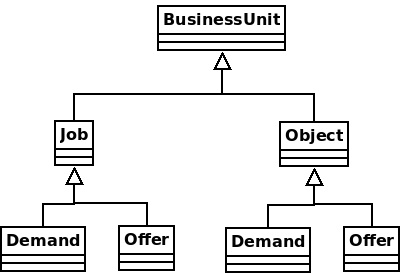
\includegraphics[scale=0.75]{modelsBU2.png}}
\end{center}
\vspace{1cm}

On remarque tout de suite que les classes Offre et Demande sont redondantes et nous avons ainsi une solution peu efficace.  Pour la suite du développement du framework,  il serait intéressant d'abstraire les offres et demandes dans une classe,  par exemple,  Transaction.  Ainsi,  le système réaliserait des échanges de Transactions de BusinessUnits.  Le schéma donnerait ce qui suit : 
\vspace{1cm}
\begin{center}
\fbox{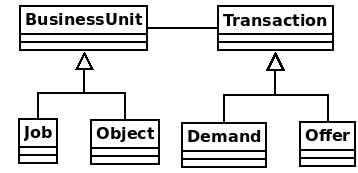
\includegraphics[scale=0.75]{newmodelsBU.png}}
\end{center}
\vspace{1cm}

Ce design permettrait de rendre le framework plus facilement adaptable pour prendre en compte l'existence,  ou non,  d'encoder des offres,  demandes,  concernant des objets ou transactions.  
\vspace{0.5cm}
Cependant,  la mise en place de ce design devrait,  selon moi,  amener un très important refactoring.  A peu près tout le code du fichier views.py (actuellement plus de 1200 lignes de code) devrait être refactoré mais pourrait amener à diminuer le nombre de classes/méthodes nécessaires à la coordination des actions.  Les templates sont également a réorganiser totalement pour pouvoir afficher correctement chaque type de transaction possible.   
\vspace{0.5cm}
 L'étape suivante peut consister en l'ajout de nouveaux features.  La méthode pour y parvenir devrait,  selon moi,  être un développement incrémental,  tel que commencé pour ce projet. En effet,  il est plus facile de suivre la démarche que nous avons décrite dans le chapitre sur le développement et ce,  pour chaque feature un par un.  Ceci semble nécessaire à la vue de la complexité du projet.  
\vspace{0.5cm}
D'une manière de plus globale,  il peut être intéressant d'envisager le concept de communauté de développeurs.  En effet,  ce framework est à destination d'organisations que l'on peut qualifier de ``transitionnaires'' et il a été développé sous licence open-source.  Ainsi,  ce serait une belle opportunité qu'un groupement se crée autour du framework afin d'une part pouvoir soutenir les organisations locales qui désirent instancier le framework,  et d'autre part,  développer de nouveaux features.  Il s'agit là,  selon moi,  d'une piste intéressante pour que ce projet soit utile à la société et utilisé par un maximum de projets locaux.  


\newpage
\section{Conclusion}

Arrivé à la fin de ce projet,  il est temps de faire le bilan des contributions de ce mémoire.  Tout d'abord,  la première partie de ce travail a consisté en une bonne dose d'analyse.  En effet,  le domaine des économiqes locales de partage est assez varié et quelques exemples de projets existants ont été repris dans le chapitre dédié à l'explication du problème.  Cette diversité a permis de donner du sens à la réalisation d'un framework plutôt qu'un projet plus classique.  En effet,  le framework offre plus de possibilités de personnalisation qu'un logiciel paramétrable,  tel que Cyclos.  Cette première étape d'analyse apporte un résultat intéressant pour le futur : un modèle des features réutilisable pour tout projet lié à ce domaine.  En effet,  cette analyse peut tout à fait être réutilisée et adaptée en vue de servir à la rédaction d'un cahier des charges d'un projet informatique.  Les définitions des features peuvent amener une première description des fonctionnalités nécessaires et le dictionnaire des termes est également une bonne source d'introduction au domaine.   
Lors du développement proprement dit,  les deux outils utilisés peuvent être considérés comme indispensables pour mettre en place un projet de cette ampleur.  En effet,  pour développer un framework,  une première étape de rétro-ingénierie est nécessaire.  D'autant plus dans notre cas puisque nous avons développé un framework destiné au web,  et donc organisé en couches composées de classes et méthodes qui s'entre-mêlent.  Ainsi,  pouvoir utiliser le debugger à des endroits clés ainsi que le script de recherche de mots clés semble indispensable.  

D'un point de vue temporel du déroulement du projet,  on distingue clairement 2 étapes : la construction du feature model d'une part,  et le développement d'autre part.  Chacune d'elle fût divisée en étapes parfois communes.  En effet,  dans les 2 cas,  il a fallut commencer par intégrer des notions théoriques.  Pour l'analyse,  il s'agissait des modèles de features,  que je ne connaissais pas auparavant.  Pour le développement,  plusieurs éléments ont dû être assimilés.  D'abord,  après avoir choisit le projet issu du groupe d'étudiants,  il a fallu s'approprier le framework Django,  ainsi que Python,  langage déjà abordé dans le cadre de certains cours mais en guise d'outil et non comme objet d'étude.  Pour Django,  le tutoriel officiel fût bien utile mais s'est malheureusement avéré insuffisant.  En effet,  une fois que l'on plonge dans le code d'un projet tel que celui qui a servi de base,  on se rend compte de la richesse de cet outil et de la complexité que l'utilisation de cette dernière peut amener.  De plus,  certains éléments du projets ou de Django en général utilisent des notions avancées de Python.  Ces 2 éléments mis ensemble m'amènent à plusieurs conclusions.  D'abord,  le développement d'un framework est plus difficile que pour un logiciel plus classique.  Dès lors,  le choix du langage qui sera utilisé par les programmeurs doit être adapté à leurs compétences.  Dans le cadre de ce projet,  la question s'est posée au moment du choix entre Cyclos et la solution du groupe d'étudiants.  Je dois bien reconnaitre que je ne m'attendais pas à devoir faire face à ce niveau de maitrise du langage.  L'autre conclusion concerne le framework Django.   En effet,  en repensant aux problèmes rencontrés pendant le développement,  je me rends compte qu'une partie était liée au fonctionnement de Django.  Dès lors,  je fais le lien avec le choix pré-cité et je pense que c'est peut-être (il faudrait mener une étude comparative pour pouvoir l'affirmer) une mauvaise idée de se baser sur un logiciel utilisant lui-même un framework,  dans le but de créer un framework pour un domaine particulier.  Je pense cela car,  lors de ce projet,  j'ai souvent été confronté à me demander si une erreur était liée à une mauvaise utilisation du langage Python ou bien de Django.  Ceci complique beaucoup la programmation,  et le problème empire si,  comme c'est mon cas,  le programmeur n'est pas expert dans au moins une des deux technologies évoquées (dans mon cas,  j'avais quelques connaissances en Python et découvrais totalement Django).  La leçon à retenir se trouve donc dans les choix qui sont posés pour ce qui servira de base au développement du framework.  Si on désire réutiliser un projet existant basé lui-même sur un framework,  il vaut mieux s'entourrer d'une équipe de connaisseurs dans les technologies liées.  Notons aussi que j'ai souligné,  au début du travail,  que le développement d'un framework se fait généralement à partir d'une solution existante.  Peut-être que ce principe peut être remis en cause si on désire absolument travailler avec un framework applicatif (c'est-à-dire qui fourni un environnement technique) et dans ce cas,  démarer le framework ``from scratch'',  pour reprendre l'expression utilisée au début de ce mémoire.

Enfin,  d'un point de vue plus personnel,  même si la difficulté rencontrée pour la programmation a été assez importante,  l'ensemble du mémoire fût aussi une belle opportunité de mettre en application de nombreux concepts abordés dans le cadre des cours de mon master en ingénierie logicielle tels que : la documentation d'une analyse de domaine,  la gestion de projets de développement informatique,  les designs patterns,  la programmation orientée objets,  etc.

En définitive,  ce travail a aussi donné des résultats intéressants dans divers domaines : l'analyse du  domaine des économies locales d'échange,  les outils pratiques pour le développement d'un framework ainsi que les bonnes pratiques de refactoring et enfin,  la conclusion que nous venons d'évoquer sur les choix faits avant de commencer la programmation.  


\appendix

\include{content/cityvisit/data}

\bibliographystyle{ThesisStyle}
\bibliography{Thesis}

%\printnomenclature

%\cleardoublepage


\end{document}
